\newpage
\section{Approximation}
Find near-optimal solutions in polynomial time

\subsection{Approximation Ratio}
\begin{definition}
    An algorithm has an \textcolor{light_blue}{approximation ratio} of  $\rho(n)$ if $\forall$input of size $n$, the cost $C$ of the solution produced by the algorithm is within a factor of $\rho(n)$ of the cost $C^*$ of an optimal solution:
    \begin{align*}
        \max\left( \frac{C}{C^*}, \frac{C^*}{C} \right)\le \rho(n)
    \end{align*}

    If an algorithm achieves an approximation ratio of $\rho(n)$, we call it a \textcolor{light_blue}{$\rho(n)$-approximation algorithm}.
\end{definition}

\begin{definition}
    An \textcolor{light_blue}{approximation scheme} for an optimization problem is an approximation algorithm that takes as input not only an instance of the problem, but also a value $\textcolor{light_red}{\varepsilon} > 0$ such that $\forall$fixed $\varepsilon$, the scheme is a \textcolor{light_red}{$(1+ \varepsilon)$-approximation algorithm}.

    We say that an approximation scheme is a \textcolor{light_blue}{polynomial-time approximation scheme (PTAS)} if $\forall$ fixed $\varepsilon > 0$, the scheme runs in time polynomial in the size n of its input instance.
\end{definition}
e.g. 
\begin{itemize}\small
    \item PTAS: $O(n^{2/\varepsilon})$, 
    \item Fully polynomial-time approximation scheme (FPTAS): $O((1/\varepsilon)^2n^3)$(关于$(1/\varepsilon)$和$n$都是多项式级的)
\end{itemize}
\subsection{Approximate Bin Packing}
Given $N$ items of sizes  $S_1 , S_2 , \dots, S_N$ , such that $0 < S_i \le 1$ $\forall$  $1 \le i \le N$.  Pack these items in the fewest number of bins, each of which has unit capacity.

\subsubsection{Next Fit}
\begin{theorem}
    Let $M$ be the optimal number of bins required to pack a list $I$ of items.  Then next fit never uses more than $2M – 1$ bins.  There exist sequences such that next fit uses $2M  – 1$ bins.
\end{theorem}

\subsubsection{First FIt}
\begin{theorem}
    Let $M$ be the optimal number of bins required to pack a list I of items.  Then first fit never uses more than $17M / 10$ bins. There exist sequences such that first fit uses $17(M – 1) / 10$ bins.
\end{theorem}

\subsubsection{Best Fit}
Place a new item in the tightest spot among all bins.

$T = O( N log N )$ and bin no.$\le  1.7M$  


\subsubsection{On-line Algorithms}
Place an item before processing the next one, and cann't change decision.

\begin{theorem}
    There are inputs that force any on-line bin-packing algorithm to use at least $\frac{5}{3}$ the optimal number of bins.
\end{theorem}

\subsubsection{Off-line Algorithms}
View the entire item list before producing an answer.

\begin{theorem}
    Let $M$ be the optimal number of bins required to pack a list $I$ of items.  Then first fit decreasing never uses more than $11M / 9 + 6/9$ bins.  There exist sequences such that first fit decreasing uses $11M / 9 + 6/9$ bins.
\end{theorem}

\subsection{The Knapsack Problem}
\subsubsection{fractional version}
A knapsack with a capacity  $M$  is to be packed.  Given $N$ items.  Each item  $i$  has a weight  $w_i$  and a profit  $p_i$ .  If  $x_i$ is the percentage of the item $i$  being packed,  then the packed profit will be  $p_i x_i$ .

An optimal packing is a feasible one with maximum profit (maximum profit density $\frac{p_i}{w_i}$).  That is,  we are supposed to find the values of $x_i$  such that $\displaystyle \sum_{i=1}^np_i x_i$ obtains its maximum under the constrains
\begin{align*}
    \sum_{i=1}^n w_i x_i \le M
\end{align*}
$x_i\in[0,1]$ for $1\le i\le n$. 


\subsubsection{0-1 version}
$x_i$ is either 1 or 0. 

The approximation ratio is 2 if we are greedy on taking the maximum profit or profit density. 

\subsubsection{Dynamic Programming Solution}
$W_{i, p}$ is the minimum weight of a collection from $\{1, \dots, i \}$ with total profit being  exactly $p$. 
\begin{align*}
    W_{i,p}=\left\{ \begin{array}{ll}
        \infty & i=0\\
        W_{i-1, p} & p_i>p\\
        \min\{ W_{i-1, p}, w_i+W_{i-1, p-p_i} \} & \text{otherwise}
    \end{array} \right.
\end{align*}
$i=1,\dots,n$, $p=1,\dots,np_{max}$. $O(n^2 p_{max})$

If $p_{max}$ is large, can round all profit values up to lie in smaller range. 
\begin{align*}
    \forall \text{ feasible solution }P, (1+\varepsilon)P_{alg}\le P
\end{align*}
$\varepsilon$ is precision parameter. 


\subsection{The K-center Problem}
\begin{figure}[!htb]
    \centering
    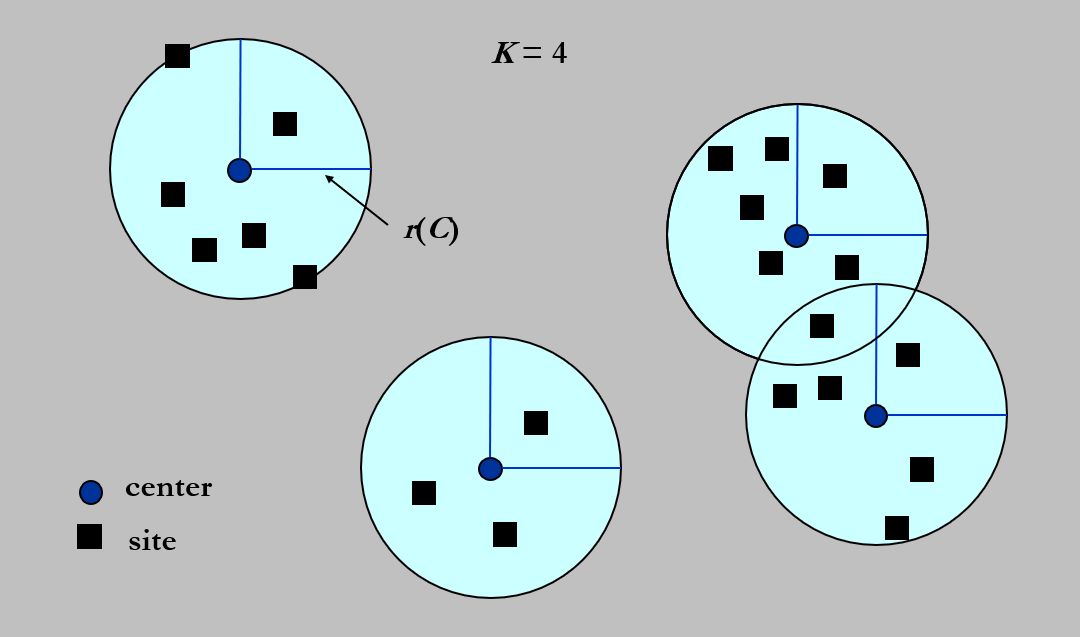
\includegraphics[width=0.42\textwidth]{pic/ADS11/K-center Problem.png}
    \caption{K-center Problem}
\end{figure}

\begin{itemize}
    \item Input: Set of $n$ sites $s_1, \dots, s_n$
    \item Center selection problem: Select $K$ centers $C$ so that the maximum distance from a site to the nearest center is minimized.
\end{itemize}

\subsubsection{Distance}
\begin{enumerate}
    \item  $dist(x, x) = 0$ (identity)
    \item $dist(x, y) = dist(y, x)$ (symmetry)
    \item $dist(x, y) \le dist(x, z) + dist(z, y)$ (triangle inequality)
\end{enumerate}
\begin{align*}
    dist(s_i , C) &= \min_{c\in C} dist(s_i, c)  \\
    &= \text{distance from $s_i$ to the closest center}\\
    r(C) &= \max_i dist(s_i, C) \\
    &= \text{smallest covering radius}
\end{align*}

Target: Find a set of centers $C$ that minimizes $r(C)$, subject to $|C| = K$.


\subsubsection{A Greedy Solution}
If we know that $r(C^*) \le r$ where $C^*$ is the optimal solution set, and choose center at  the site, we can verify whether $r$ meets the requirements. 

\begin{lstlisting}[language={c++}]
Centers Greedy-2r(Sites S[], int n, int K, double r){
    Sites  S_[]=S[]; /* S_ is the set of the remaining sites */
    Centers C[]={};
    while(!S_.empty){
        Select any s from S_ and add it to C;
        Delete all s_ from S_ that are at dist(s_, s) `$\le$` 2r;
    } /* end-while */
    if (|C|<=K) return C;
    else ERROR(No set of K centers with covering radius at most r);
}
\end{lstlisting}
\begin{theorem}
    Suppose the algorithm selects more than $K$ centers.  Then for any set $C^*$ of size at most $K$, the covering radius is $r(C^*) > r$.
\end{theorem}


Binary search for $r$ to know $r(C^*)$. Solution radius is $2r_1$ --- 2-approximation. 

Or
\begin{lstlisting}[language={c++}]
Centers Greedy-Kcenter(Sites S[], int n, int K){
    Centers  C[] = {};
    `Select any s from S and add it to C`;
    while (|C|<K) {
        `Select s from S with maximum dist(s, C)`;
        Add s it to C;
    } /* end-while */
    return C;
}
\end{lstlisting}
\begin{theorem}
    The algorithm returns a set $C$ of $K$ centers such that $r(C) \le 2r(C^*)$ where $C^*$ is an optimal set of $K$ centers.(2-approximation)
\end{theorem}

\begin{theorem}
    Unless P = NP, there is no  $\rho$-approximation for center-selection problem for any $\rho < 2$.
\end{theorem}

\subsection{Three aspects to be considered}
\begin{itemize}
    \item A: Optimality(quality of a solution
    )
    \item B: Efficiency(cost of computations)
    \item C: All instances 
\end{itemize}

Researchers are working on
\begin{itemize}
    \item A+C: Exact algorithms for all instances
    \item A+B: Exact and fast algorithms for special cases
    \item B+C: Approximation algorithms 
\end{itemize}
Even if P=NP, still we cannot guarantee A+B+C .
